\documentclass{article}
\usepackage[utf8]{inputenc}
\usepackage{graphicx}
\usepackage{listings}
\usepackage{comment}

\title{Data Mining}
\author{AmirHossein Vatanibaf}

%Here begins the body of the document
\begin{document}
\maketitle

\section{Introduction}
"Statistical thinking will one day be as necessary for efficient citizenship as is the ability to read and write"

          H.G. Wells   Circa  1925

\section{Data Mining}
Data mining is the process of finding anomalies, patterns and correlations within large data sets to predict outcomes. Using a broad range of techniques, you can use this information to increase revenues, cut costs, improve customer relationships, reduce risks and more.

\begin{figure}
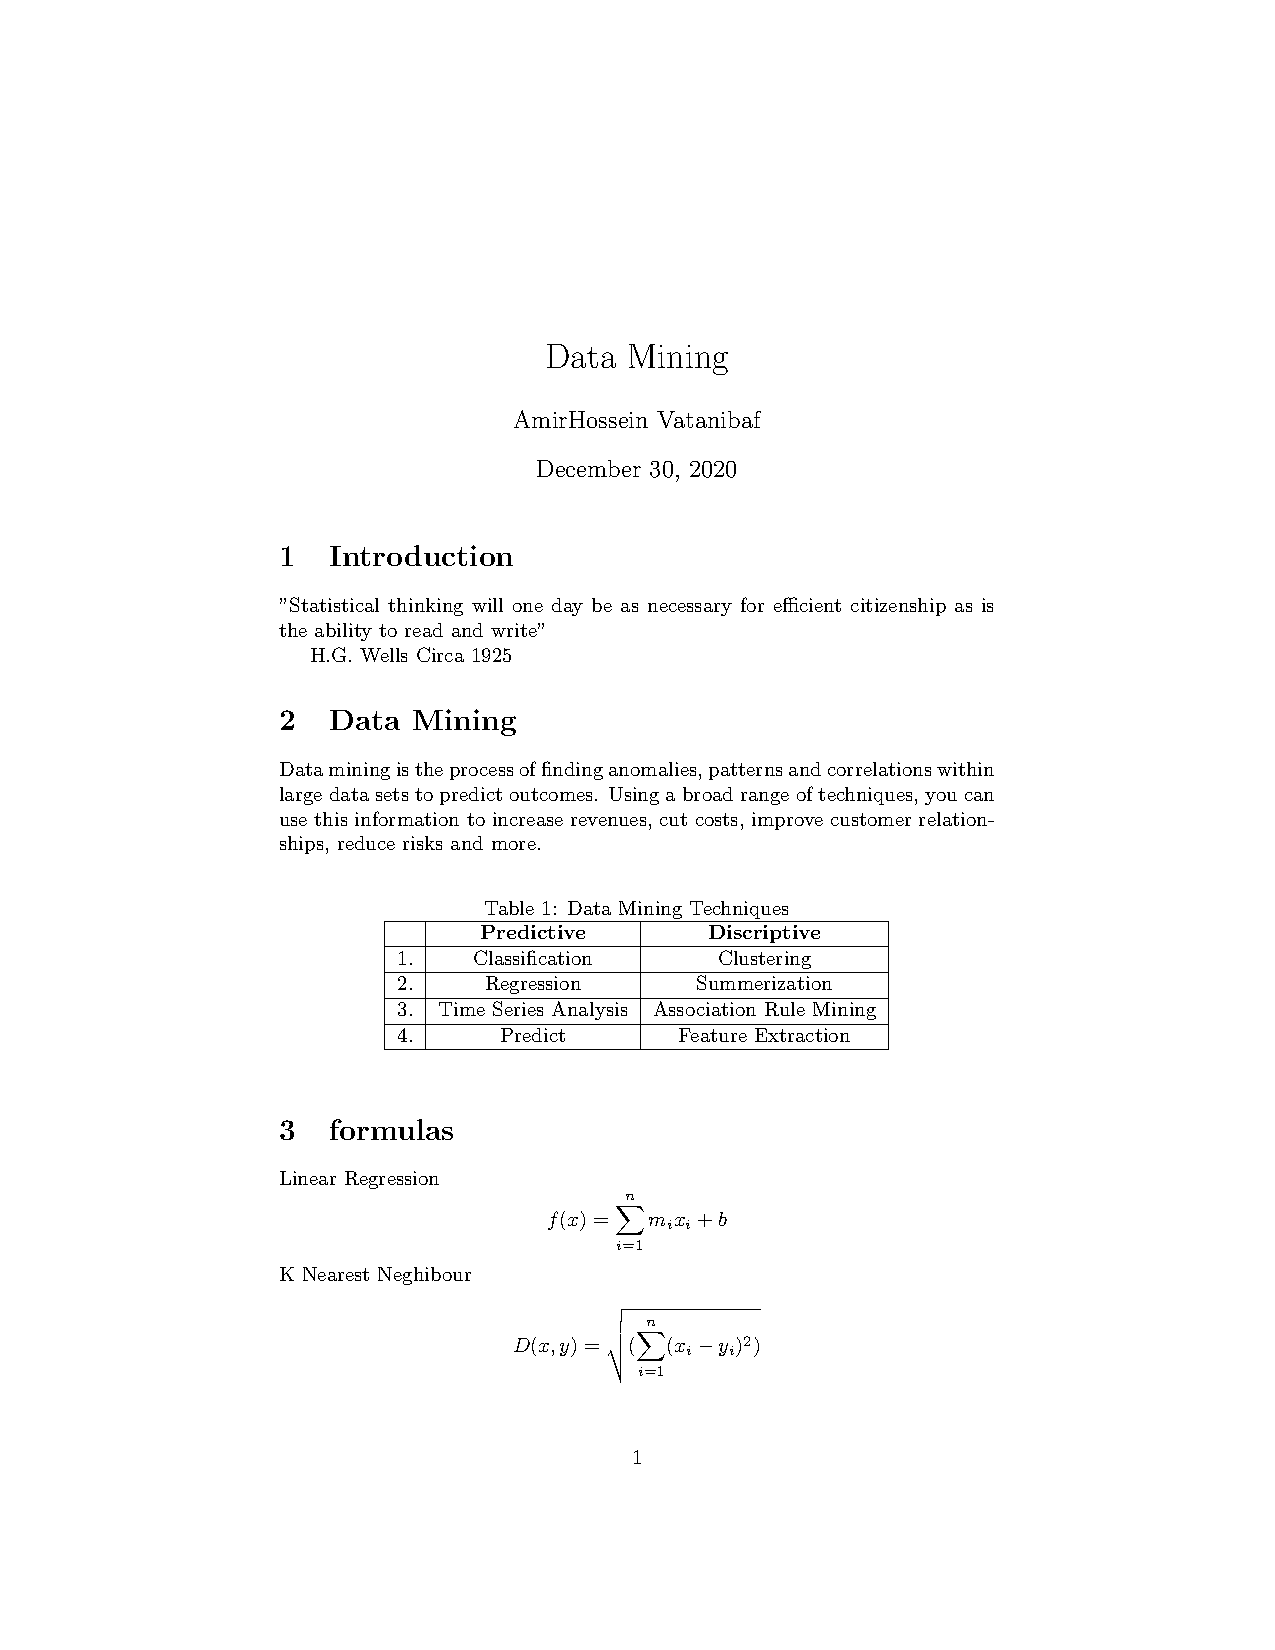
\includegraphics[width=11cm]{Data Mining.jpg}
\begin{center}
\caption{A List Of Top Data Mining Algorithms}
\end{cneter}
\end{figure}

\begin{table}[h!]
  \begin{center}
    \caption{Data Mining Techniques}
    \label{tab:table1}
    \begin{tabular}{|c|c|c|c|} 
    \hline
      \textbf{} & \textbf{Predictive} & \textbf{Discriptive}\\
    
      \hline
      1. & Classification & Clustering \\
     \hline
      2. & Regression & Summerization \\
      \hline
      3. & Time Series Analysis & Association Rule Mining \\
      \hline
      4. & Predict & Feature Extraction \\
      \hline
    \end{tabular}
  \end{center}
\end{table}

\section{formulas}
Linear Regression $$ f(x) = \sum^{n}_{i=1} m_ix_i + b $$  
K Nearest Neghibour  $$ D(x,y)= \sqrt{ (\sum^{n}_{i=1} (x_i - y_i )^2)} $$

\section{Code Example with cpp,Program BFS Algorithm }
\lstinputlisting{BFS-code.cpp}

\end{document}